%\externaldocument[-f]{c2_foundations}
\appendix

\chapter{Amalgamation Operation}
\label{ap:amalgamation}
A CTBN with multiple variables can be represented with a single CIM. This is done by amalgamation operation. Amalgamation defines a combining operation over multiple CIMs and produces a single CIM for the entire system. \cite{Nodelman1995}

\section{Amalgamation of Independent Processes}
Consider a CTBN with graph $ \mathcal{G} = \left\lbrace \mathcal{V}, \mathcal{E} \right\rbrace $ over two variables such that $ \mathcal{V} = \left\lbrace X_1, X_2\right\rbrace $. Assume variables $ X_1 $ and $ X_2 $ with intensity matrices $ \textbf{Q}_1 $ and $ \textbf{Q}_2 $, are both parent nodes, i.e. $ \mathcal{E} = \emptyset $ and $ Par_{\mathcal{G}}(X_1) = Par_{\mathcal{G}}(X_1) = \emptyset $. This CTBN can be identified as a subsytem of the CTBN model described in \cref{sec:exp_ctbn_model}. \\
Analogous to \autoref{eq:Markov_trans_func}, Markov transition function for the joint process can be derived as
\begin{align}
	\operatorname{Pr}(X_P(t+h) = x_p^\prime\mid X_P(t) = x_p)
	&=  \operatorname{Pr}(X_1(t+h) = x_1^\prime, X_2(t+h) = x_2 \mid X_1(t) = x_1, X_2(t) = x_2)\nonumber \\
	&= \operatorname{Pr}(X_1(t+h) = x_1^\prime \mid X_1(t) = x_1, X_2(t) = x_2) \nonumber\\
	& \quad \quad \quad \operatorname{Pr}( X_2(t+h) = x_2 \mid X_1(t) = x_1, X_2(t+h) = x_2) \nonumber\\
	& = (\delta_{x_1^\prime, x_1} + hq^1_{x_1, x_1^\prime} + o(h))(1 + hq^2_{x_2, x_2} + o(h))\nonumber\\
	& = \delta_{x_1^\prime, x_1} + hq^1_{x_1, x_1^\prime} + h\delta_{x_1^\prime, x_1}q^2_{x_2, x_2} + o(h)
	\label{eq:amalg}
\end{align}
where $ x_1, x_1^\prime \in \rchi_1 $, $ x_2, x_2^\prime \in \rchi_2 $, $ x_p = (x_1, x_2), x_p^\prime = (x_1^\prime, x_2) \in \rchi_P $.\\
Suppose the intensity matrices of $ X_1 $ and $ X_2 $ are in the form
\begin{equation}
\textbf{Q}_i = 
\begin{bmatrix}
-q^{i}_{0} & q^{i}_{0} \\
q^{i}_{1} & -q^{i}_{1}
\end{bmatrix} \quad \text{for } i \in \left\lbrace 1,2\right\rbrace 
\end{equation}
Then the intensity matrix for the joint process $ X_P $ with factorising state space $ \rchi_P = \rchi_1 \times \rchi_2 $ can be written as
\begin{equation}
\textbf{Q}_P = 
\begin{bmatrix}
-q^{2}_{0}-q^{1}_{0} & q^{2}_{0} & q^{1}_{0} & 0 \\
q^{2}_{1} & -q^{2}_{1}-q^{1}_{0} & 0 & q^{1}_{0} \\
q^{1}_{1} & 0 & -q^{1}_{1}-q^{2}_{0} & q^{2}_{0} \\
0 & q^{1}_{1} & q^{2}_{1} & -q^{1}_{1}-q^{2}_{1}
\end{bmatrix} \quad \text{for } i \in \left\lbrace 1,2\right\rbrace 
\label{eq:amalgamated_q}
\end{equation}
As it can be observed from \autoref{eq:amalgamated_q}, the transition intensities which corresponds to state transition in both variables, i.e. anti-diagonal entries, are zero, due to the one of the assumptions in CTBN framework that only one variable can transition at a time, as given in \cref{sec:ctbn_intro}.
%x1 = Q1[0][1]
%x2 = Q1[1][0]
%y1 = Q2[0][1]
%y2 = Q2[1][0]
%[[0, y1, x1, .0],
%[y2, 0, .0, x1],
%[x2, .0, 0, y1],
%[.0, x2, y2, 0]])
\chapter{Marginalized Likelihood Function for Homogenous Continuous Time Markov Processes}
\label{ap:marg_llh_ctmp}

Let $ X $ be a homogenous CTMP. For convenience, it is assumed to be binary-valued, $ \rchi = \left\lbrace x_{0}, x_{1} \right\rbrace $. The transition intensity matrix can be written in the following form:
\begin{equation}
\textbf{Q} = 
\begin{bmatrix}
-q_{0} & q_{0} \\
q_{1} & -q_{1}
\end{bmatrix}
\end{equation}
where the transition intensities $ q_{0} $ and $ q_{1} $ are gamma-distributed with parameters $ \alpha_{0}$, $ \beta_{0} $ and $ \alpha_{1} $, $ \beta_{1} $, respectively. The marginal likelihood of a sample trajectory $ X^{[0,T]} $ can be written as follows:
\begin{align}
P(X^{[0, T]}) & = \int  P(X^{[0, T]}\mid Q)P(Q) dQ \nonumber\\ 
& = \int_{0}^{\infty} = \prod_{j \neq i}  \exp(-q_{i,j}T[x_{i}])\ q_{i,j}^{M[x_{i},x_{j}]} \frac{\beta_{i,j}^{\alpha_{i,j}}{q_{i,j}^{\alpha_{i,j}-1}}\exp(-\beta_{i,j}q_{i,j})}{\Gamma(\alpha_{i,j})} \ dq_{i,j} \nonumber\\ 
& = \prod_{i\in{0,1}}\int_{0}^{\infty} q_{i}^{M[x_{i}]} \ \exp(-q_{i}T[x_{i}]) \  \frac{\beta_{i}^{\alpha_{i}} \ q_{i}^{\alpha_{i}-1}\ \exp(-\beta_{i}q_{i})}{\Gamma(\alpha_{i})} \ dq_{i} \nonumber\\ 
& = \prod_{i\in{0,1}} \frac{\beta_{i}^{\alpha_{i}}}{\Gamma(\alpha_{i})} \int_{0}^{\infty} q_{i}^{M[x_{i}] + \alpha_{i} -1} \ \exp(-q_{i}(T[x_{i}]+\beta_{i})) \ dq_{i} \label{eq:wolfram_line}\\ 
& = \prod_{i\in{0,1}} \frac{\beta_{i}^{\alpha_{i}}}{\Gamma(\alpha_{i})} \left( -(T[x_{i}]+\beta_{i})^{-M[x_{i}] - \alpha_{i}}\ \Gamma(M[x_{i}] + \alpha_{i}, \ q_{i}(T[x_{i}]+\beta_{i})) \right) \Big|_0^\infty  \nonumber\\ 
& = \prod_{i\in{0,1}} \frac{\beta_{i}^{\alpha_{i}}}{\Gamma(\alpha_{i})} \left( (T[x_{i}]+\beta_{i})^{-M[x_{i}] - \alpha_{i}}\ \Gamma(M[x_{i}] + \alpha_{i}) \right)
\label{eq:Marg_traj}
\end{align}
%where $ T[x_{i}] $, the amount of time spent in state x, $ M[x,x'] $ the number of transitions from state x to x' and  $ M[x] = \sum_{x\neq x'}M[x,x'] $.\\

In \autoref{eq:wolfram_line}, the integral is solved using computer algebra system WolframAlpha as follows:
\begin{align}
\int x^{a} \ \exp(-xb) \ dx = -b^{-a-1} \ \Gamma(a+1, \ bx) + C
\label{eq:integral}
\end{align}

\chapter{Equivalence Classes of Observation Models}
\label{ap:eq_classes}
The equivalence classes are inherent to the problem setting and caused by two reasons. In this chapter, these reasons are explained and illustrated.
\section*{Identical Effect on Belief State}
Some observation models fall into the same class due to their exact same effect on the belief state. An example of this situation is illustrated in ..... In order to show the exact equivalence, the simulations are performed belief state update using exact update method as described in \cref{par:bs_exact}. Consider the problem of calculating the likelihood of one sample $ S^{[0,T]} $ given two observation models, $ \psi_1 $ and $ \psi_2 $ given below. Given a sample of parent trajectories shown in ....., it is obvious that these two observation models lead to different observation trajectories as shown in ... and ..... Nonetheless, using \autoref{eq:bs_exact}, the resulting belief state is exactly the same. This leads to the exact same trajectories for $ Q_3 $ and the likelohood of the sample given these two observation models, $ p(S^{[0,T]} \mid \psi_1 ) $ and $ p(S^{[0,T]} \mid \psi_2 ) $ end up exactly same. %TODO
\begin{figure}[H]
	\begin{center}
		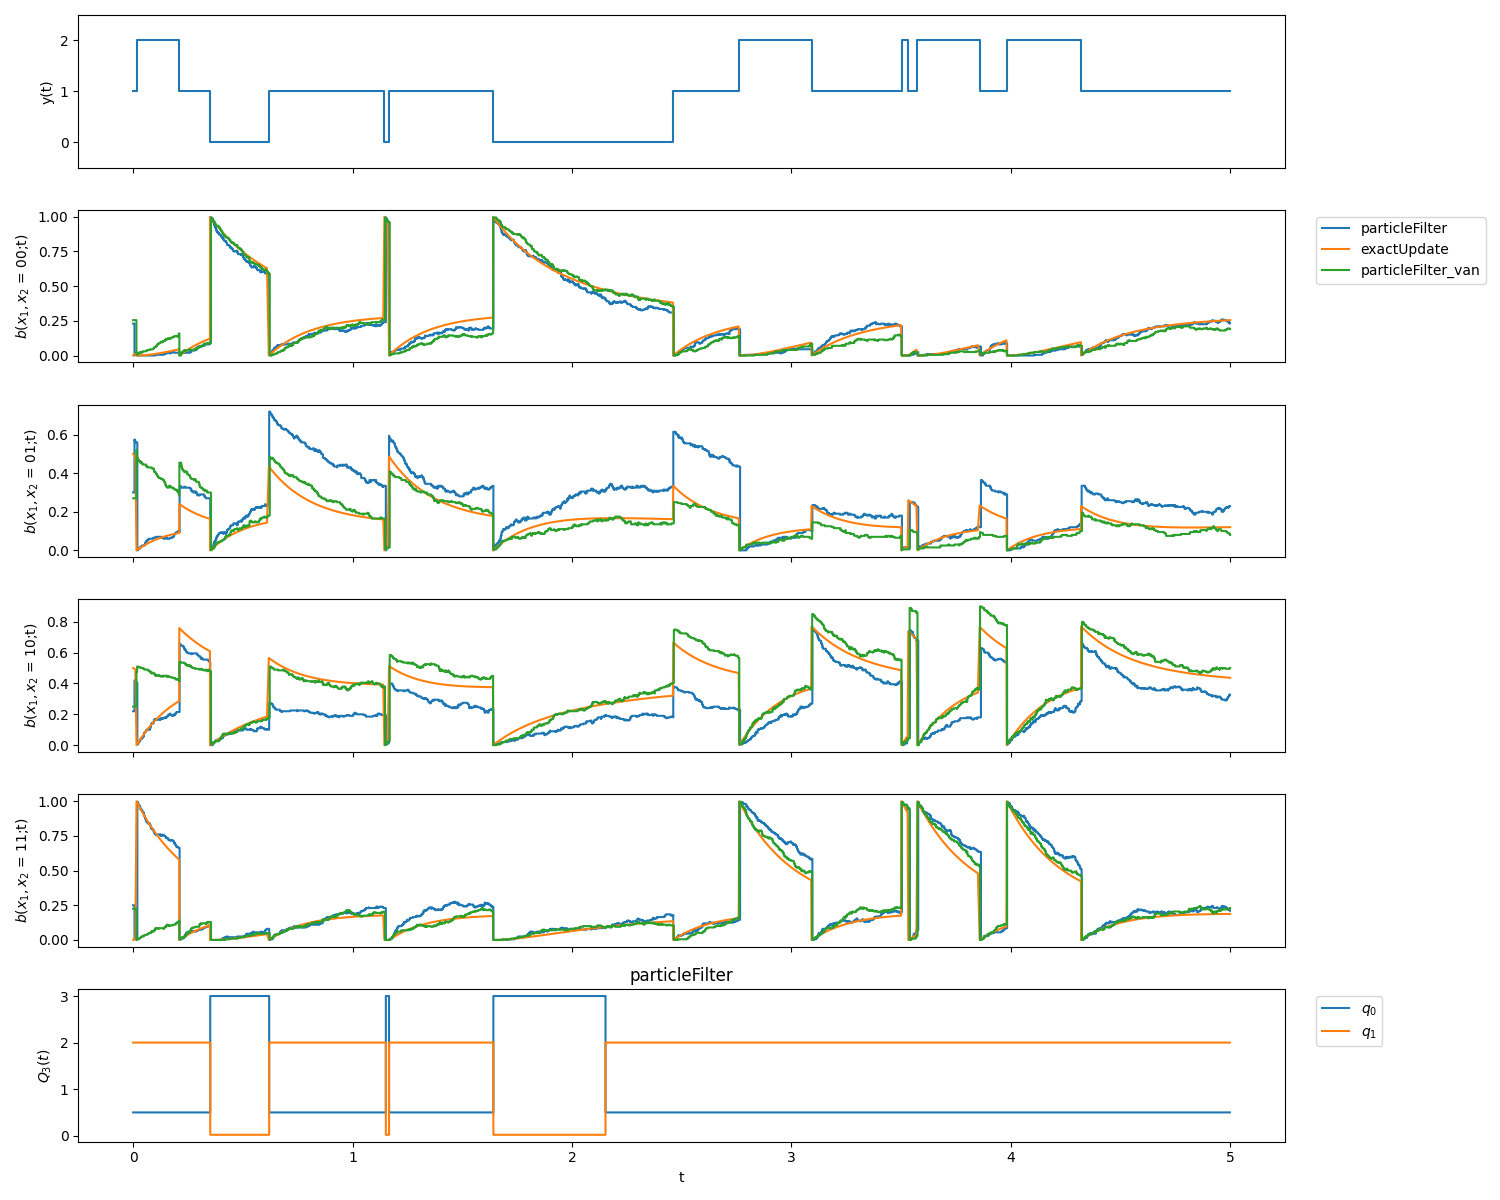
\includegraphics[width=.60\textwidth]{figures/b_q_traj}
		\caption{Belief state and $ Q_3 $ trajectories}
		\label{fig:b_q_traj}
	\end{center}
\end{figure}
\begin{align}
p(S^{[0,T]} \mid \psi_2 ) &= \\
p(S^{[0,T]} \mid \psi_2 ) &=
\label{eq:integral}
\end{align}
\section*{Combination of Belief State and Policy}
For some observation model, the reason of equivalence is that even though the belief state are different, the policy $ \pi(b) $ leads to same trajectory for $ Q_3 $. This case is exemplified in ..... where the simulations are performed belief state update using exact update method as described in \cref{par:bs_exact}. Consider the problem of calculating the likelihood of one sample $ S^{[0,T]} $ given two observation models, $ \psi_1 $ and $ \psi_2 $ given below. Given a sample of parent trajectories shown in .....,  these observation models lead to different observation trajectories as shown in ... and ....., which results in different belief state trajectories given in ..... However, the behaviour of the agent is dominated by ...., and the policy leads to the exact same trajectories for $ Q_3 $ and the likelohood of the sample given these two observation models, $ p(S^{[0,T]} \mid \psi_1 ) $ and $ p(S^{[0,T]} \mid \psi_2 ) $ end up exactly same. %TODO
\begin{figure}[H]
	\begin{center}
		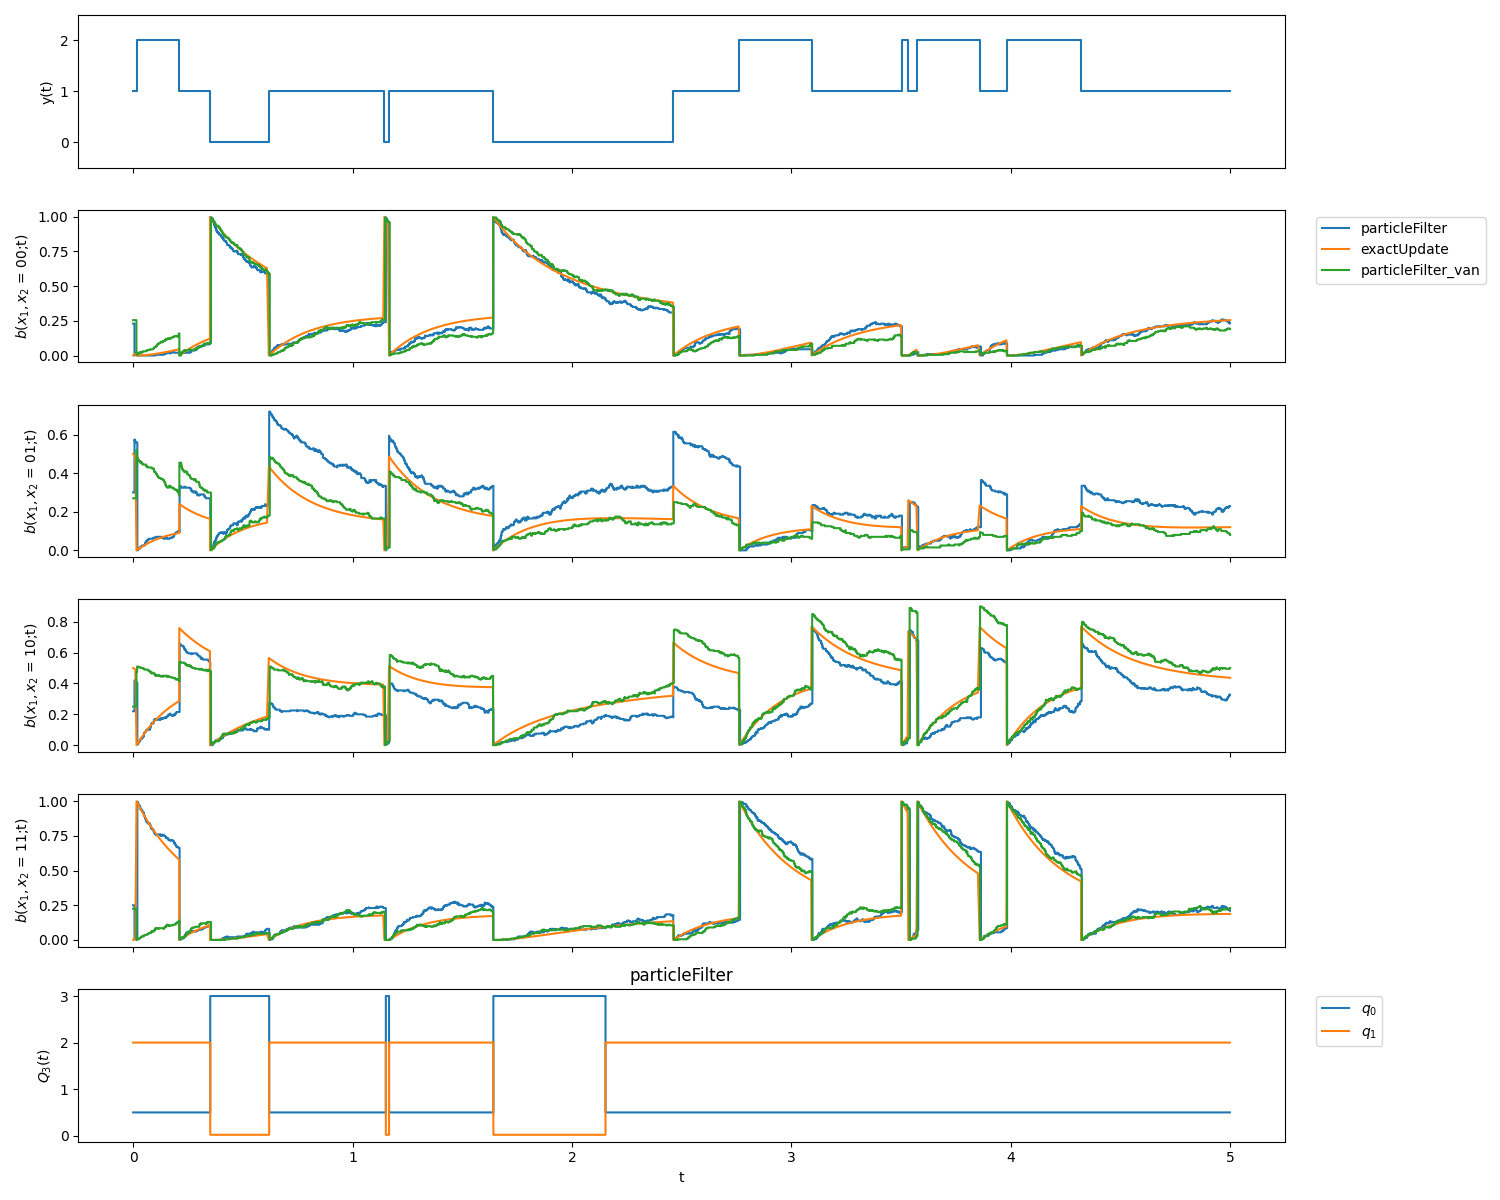
\includegraphics[width=.60\textwidth]{figures/b_q_traj}
		\caption{Belief state and $ Q_3 $ trajectories}
		\label{fig:b_q_traj}
	\end{center}
\end{figure}
\begin{align}
p(S^{[0,T]} \mid \psi_2 ) &= \\
p(S^{[0,T]} \mid \psi_2 ) &=
\label{eq:integral}
\end{align}
\section{Observation Models in Experiments}
As mentioned in \cref{sec:eq_classes}, the inference problem is reduced to maximum likelihood estimation between 10 classes. One observation model is picked as as representative of each classes and considered for the inference problem. These observation models are given below.
\begin{align}
\psi_{\text{true}} = \psi_{0} &=
\begin{bmatrix}
1 & 0 & 0 \\
0 & 1 & 0 \\
0 & 1 & 0 \\
0 & 0 & 1
\end{bmatrix}
\psi_{1} =
\begin{bmatrix}
1 & 0 & 0 \\
0 & 1 & 0 \\
0 & 1 & 0 \\
0 & 0 & 1
\end{bmatrix}
\psi_{2} =
\begin{bmatrix}
1 & 0 & 0 \\
0 & 1 & 0 \\
0 & 1 & 0 \\
0 & 0 & 1
\end{bmatrix}
\psi_{3} =
\begin{bmatrix}
1 & 0 & 0 \\
0 & 1 & 0 \\
0 & 1 & 0 \\
0 & 0 & 1
\end{bmatrix}
\psi_{4} =
\begin{bmatrix}
1 & 0 & 0 \\
0 & 1 & 0 \\
0 & 1 & 0 \\
0 & 0 & 1
\end{bmatrix} \\
\psi_{5} &=
\begin{bmatrix}
1 & 0 & 0 \\
0 & 1 & 0 \\
0 & 1 & 0 \\
0 & 0 & 1
\end{bmatrix}
\psi_{6} =
\begin{bmatrix}
1 & 0 & 0 \\
0 & 1 & 0 \\
0 & 1 & 0 \\
0 & 0 & 1
\end{bmatrix}
\psi_{7} =
\begin{bmatrix}
1 & 0 & 0 \\
0 & 1 & 0 \\
0 & 1 & 0 \\
0 & 0 & 1
\end{bmatrix}
\psi_{8} =
\begin{bmatrix}
1 & 0 & 0 \\
0 & 1 & 0 \\
0 & 1 & 0 \\
0 & 0 & 1
\end{bmatrix}
\psi_{9} =
\begin{bmatrix}
1 & 0 & 0 \\
0 & 1 & 0 \\
0 & 1 & 0 \\
0 & 0 & 1
\end{bmatrix}
\end{align}

\chapter{Additional Results}